\documentclass{article}
\usepackage[utf8]{inputenc}
\usepackage[papersize={8.5in,11in},margin=0.8in]{geometry}
\usepackage{adjustbox}
\usepackage{xcolor}
\usepackage{color, colortbl}
\usepackage{graphicx}
\definecolor{LightCyan}{rgb}{0.88,1,1}
\definecolor{LightRed}{rgb}{1,0.49,0.49}
\usepackage{amsfonts}
\usepackage{amsmath}
\usepackage{amssymb}
\usepackage{tikz}
\usetikzlibrary{positioning}
\usetikzlibrary{graphs,graphs.standard}

\title{MATH 505 Final Exam}
\author{John Caruthers}
\date\today

\begin{document}
\maketitle

\textbf{I have neither given nor received any unauthorized aid on this exam.} \\\hspace*{1cm}“Signature:” John Caruthers

\begin{itemize}
    \item[1.] Consider the argument below.
    
    If a tree loses its leaves, it is cold outside.\\
    It is cold outside.\\
    ----------------------------------------------- \\
    Therefore, the tree loses its leaves.
    \begin{itemize}
        \item[a.] Write the argument symbolically.  Be sure to denote what your symbols represent.\\
        {\color{blue}
        $p:$ A tree loses its leaves\\
        $q:$ It is cold outside
        
        \hspace*{1cm}$p\to q$\\
        \hspace*{1cm}$q$\\
        \hspace*{1cm}-------- \\
        \hspace*{1cm}$\therefore p$}
        
        \item[b.] Is the argument valid or not? Explain.
        
        An argument is valid if the conclusion is true every time the conjunction of the premises is true.  A truth table can be build to check:
        \begin{center}
            \begin{tabular}{|c|c|c|c|c|}
                \hline
                $p$ & $q$ & $p\to q$ & $(p\to q)\wedge q$ & $p$ \\
                \hline
                \rowcolor{LightCyan}
                T & T & T & T & T\\
                \hline
                T & F & F & F & T\\
                \hline
                \rowcolor{LightRed}
                F & T & T & T & F\\
                \hline
                F & F & T & F & F\\
                \hline
            \end{tabular}
        \end{center}
        {\color{blue}There are two instances where the conjunction of the premises is true, one of those has a false conclusion, therefore the argument is not valid.}
    \end{itemize}
    
    \item[2.] Produce a truth table for the following statement: $(p\wedge\sim q)\to(\sim r\vee p)$
    \begin{center}
        \begin{tabular}{|c|c|c|c|c|c|c|c|}
            \hline
            $p$ & $q$ & $r$ & $\sim q$ & $\sim r$ & $p\wedge \sim q$ & $\sim r\vee p$ & $(p\wedge \sim q)\to(\sim r\vee p)$\\
            \hline
            T & T & T & F & F & F & T & T\\
            \hline
            T & T & F & F & T & F & T & T\\
            \hline
            T & F & T & T & F & T & T & T\\
            \hline
            T & F & F & T & T & T & T & T\\
            \hline
            F & T & T & F & F & F & F & T\\
            \hline
            F & T & F & F & T & F & T & T\\
            \hline
            F & F & T & T & F & F & F & T\\
            \hline
            F & F & F & T & T & F & T & T\\
            \hline
        \end{tabular}
    \end{center}
    
    \item[3.] Consider the sequence that begins: $4, 10, ...$
    \begin{itemize}
        \item[a.] If the sequence is arithmetic, what are the next 3 terms? {\color{blue}$16, 22, 28$}
        \newpage
        \item[b.] If the sequence is arithmetic, what is the formula for $a_n$?\\ {\color{blue}Using the equation $a_n=a_1+(n+1)d$, with $a_1=4$, $d=6$:
        \begin{align}
            a_n&=4+6(n-1)\nonumber\\
            a_n&=4+6n-6\nonumber\\
            a_n&=6n-2\nonumber
        \end{align}}

        \item[c.] If the sequence is geometric, what are the next 3 terms? {\color{blue}$25, \frac{125}{2}, \frac{625}{4}$}
        \item[d.] If the sequence is geometric, what is the formula for $a_n$?\\
        {\color{blue}Using the formula $a_n=a_1\cdot r^{n-1}$, with $r=\frac{5}{2}$ and $a_1=4$
        \begin{align}
            a_n=4\cdot\left[ \frac{5}{2} \right]^{n-1}\nonumber
        \end{align}}
    \end{itemize}
    
    \item[4.] Let $x$ be an even integer and let $y$ and $z$ be odd integers.  Prove that $xy+z$ is an odd integer.
    
    \textbf{Direct proof}: Assume $x,y,z \in \mathbb{Z}$. $x$ is even integer and can be represented by $2j$, $y$ is an odd integer and can be represented by $2k+1$, $z$ is an odd integer and can be represented by $2i+1$ with $j,k,i \in \mathbb{Z}$. Input these representations into $xy+z$ and show that it is an odd integer of form $2r+1$ with $r \in \mathbb{Z}$.
    \begin{align}
        xy+z&=2r+1\nonumber\\
        (2j)(2k+1)+(2i+1)&=2r+1\nonumber\\
        4jk+2j+2i+1&=2r+1\nonumber\\
        2(2jk+j+i)+1&=2r+1\nonumber
    \end{align}
    Represent $2jk+j+i$ with integer $r$ per Axiom of Integers.
    \begin{align}
        2r+1&=2r+1\nonumber
    \end{align}
    {\color{blue}It is proven that $xy+z$ is an odd integer with $x$ being even and $y,z$ being odd.} $\blacksquare$
    
    \item[5.] For all positive integers $n$, prove that $5$ divides $9^n-4^n$.
    
    \textbf{Proof by Induction}: Assume 5 divides into itself and any number multiplied by itself.
    \begin{itemize}
        \item[]\emph{Basis:} Set $n=1$
        \begin{align}
            5&|\left(9^1-4^1\right)\nonumber\\
            5&|(9-4)\nonumber\\
            5&|5\nonumber
        \end{align}
        
        \item[]\emph{Inductive Hypothesis:} Set $n=k$ such that $k\in\mathbb{Z}$.
        \begin{align}
            5&|\left(9^k-4^k\right)\nonumber
        \end{align}
        
        \item[]\emph{Inductive Step:} Set $n=k+1$ such that $k\in\mathbb{Z}$. Assume Inductive Hypothesis is true, show that Inductive Step is true.
        \begin{align}
            5&|\left( 9^{k+1}-4^{k+1}\right)\nonumber\\
            5&|\left(9\cdot9^k-4^{k+1}\right)\nonumber\\
            5&|\left((5+4)9^k-4^{k+1}\right)\nonumber\\
            5&|\left(5\cdot9^k+4\cdot9^k-4^{k+1}\right)\nonumber\\
            5&|\left(5\cdot9^k+4\cdot9^k-4\cdot4^k\right)\nonumber\\
            5&|\left(5\cdot9^k+4\left(9^k-4^k\right)\right)\nonumber
        \end{align}
        {\color{blue}Since 5 divides into any number multiplied by 5, 5 divides into $9^k-4^k$, and 5 divides into the sum of these numbers, it is proven by induction, that 5 divides $9^n-4^n$ for all positive integers $n$.} $\blacksquare$
    \end{itemize}
    
    \item[6.] Prove by induction: If $S$ is a set with $n$ elements, then $S$ has $2^n$ distinct subsets.
    \begin{itemize}
        \item[]\emph{Basis:} Set $n=0$, a set $S$ with $0$ elements has $2^0=1$ subsets.  This subset is the empty set: $\emptyset$.
        
        \item[]\emph{Inductive Hypothesis:} Set $n=k$, a set $S$ with $k$ elements has $2^k$ subsets.
        
        \item[]\emph{Inductive Step:} Set $n=k+1$, a set $S$ with $k+1$ elements has $2^{k+1}$ subsets.  Imagine the set $S_1$ with $k$ elements and has $2^k$ subsets.  $S_1=S-\{a\}$ where $\{a\}$ is an arbitrary element in $S$. For each subset of $S$, there are $2^k$ subsets without the element $a$, and $2^k$ subsets that contain the element $a$.  This means that there are $2\cdot2^k$ elements or $2^{k+1}$ elements in $S$. This means that adding another element to a $S_1$ means there are $2^{k+1}$ subsets. $\blacksquare$
    \end{itemize}
    
    \item[7.] Use the Geometric Shortest-Path Algorithm to find the most efficient path from vertex $A$ to vertex $Z$.  You do not need to explain all your steps but give \emph{two intermediate steps} in the process.
    \begin{figure}[h]
        \centering
        \includegraphics[width=0.45\textwidth]{Q7_1.png}
    \end{figure}
    
    Use table to decide next node to travel to.
    \begin{center}
        \begin{tabular}{cc}
            Edges & Length\\
            \hline
            AI & 6\\
            \rowcolor{LightCyan}
            AB & 4\\
            AB & 7\\
        \end{tabular}
    \end{center}
    Choose B as the next node
    \begin{figure}[htbp]
        \centering
        \includegraphics[width=0.45\textwidth]{Q7_2.png}
    \end{figure}
    \newpage
    Again use a table to decide next node, put previously untraveled nodes on selection list too.
    \begin{center}
        \begin{tabular}{cc}
            Edges & Length\\
            \hline
            AI & 6\\
            AB & 7\\
            BH & 9\\
            \rowcolor{LightCyan}
            BC & 6\\
        \end{tabular}
    \end{center}
    Choose C as the next node.
    \begin{figure}[htbp]
        \centering
        \includegraphics[width=0.45\textwidth]{Q7_3.png}
    \end{figure}
    
    In my selection, there were instances of paths tying for the same lengths. Randomly selecting a node in this case is suitable. Repeating the process of selecting the shortest length edges, leads to the shortest path below:
    \begin{figure}[htbp]
        \centering
        \includegraphics[width=0.45\textwidth]{Q7_4.png}
    \end{figure}
    \newpage
    \item[8.] Draw the complete graph $K_5$ and the completed bipartite graph $K_{2,3}$ and label which is which. Are these two graphs isomorphic? Explain your answer.
    \begin{center}
        $K_5$
        
        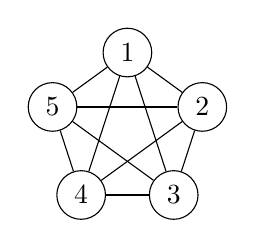
\begin{tikzpicture}[nodes={draw, circle}]
            \graph {subgraph K_n [n=5,clockwise,radius=1cm] };
        \end{tikzpicture}   
    \end{center}
    
    \begin{center}
        $K_{2,3}$
        
        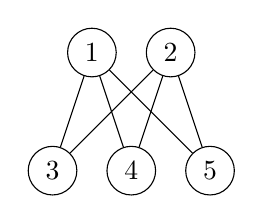
\begin{tikzpicture}
           [dot/.style = {draw,circle}]
            \node[dot] (d) at (0, -1.5) {$4$};
            \node[dot] (c) at (-1,-1.5) {$3$};
            \node[dot] (e) at (1,-1.5) {$5$};
            \node[dot] (a) at (-0.5,0) {$1$};
            \node[dot] (b) at (0.5,0) {$2$};
        
            \path[-] (a) edge (c);
            \path[-] (a) edge (d);
            \path[-] (a) edge (e);
            \path[-] (b) edge (c);
            \path[-] (b) edge (d);
            \path[-] (b) edge (e);
            
            \end{tikzpicture}
    \end{center}
    
    {\color{blue} $K_5$ and $K_{2,3}$ are not isomorphic because there is no one to one relation between any point.  For example, all the nodes in $K_5$ are of degree $4$, while none of the nodes in $K_{2,3}$ are of degree 4. }
    
    \item[9.] The Rhombicosidodecahedron is an Archimedean solid and a polyhedron with 20 regular triangular faces, 30 square faces, 12 regular pentagonal faces, and 60 vertices.  How many edges does this polyhedron have?  Briefly explain your answer.
    
    Per \emph{Euler's Theorem for Simple Polyhedra}, the relationship between faces($f$), vertices($v$), and edges($e$) is: $v-e+f=2$. Inputting the information about a Rhombicosidodecahedron into this equation lets us solve for the number of edges.
    \begin{align}
        v-e+f&=2\nonumber\\
        60-e+(20+30+12)&=2\nonumber\\
        60-e+62&=2\nonumber\\
        -e&=2-60-62\nonumber\\
        e&=120\nonumber
    \end{align}
    {\color{blue} There are 120 edges in a Rhombicosidodecahedron.}
    \newpage
    \item[10.] Consider the following expression: $(4-7)^2+5\cdot(7+3)$.
    \begin{itemize}
        \item[a.] Evaluate this expression
        \begin{align}
            &(4-7)^2+5\cdot(7+3)\nonumber\\
            &=(-3)^2+5\cdot10\nonumber\\
            &=9+50\nonumber\\
            &=59\nonumber
        \end{align}
        \item[b.] Create a binary tree that represents this expression. Label the vertices with the corresponding number or operation.
        \begin{figure}[h]
            \centering
            \includegraphics[width=0.8\textwidth]{Q10b.png}
        \end{figure}
        
        \item[c.] What is the infix form of the expression?
        
        {\color{blue}$4-7\times4-7+5\times7+3$}
        \item[d.] What is the postfix form of the expression?
        
        {\color{blue}$47-47-\times573+\times+$}
    \end{itemize}
    
    \item[11.] There are 14 juniors and 16 seniors(30 total) trying out for the varsity field hockey team. In how many ways can the team be chosen if there must be:
    \begin{itemize}
        \item[a.] A total of 16 players total on the team? {\color{blue}$\frac{30!}{(30-16)!}=3042648073975910400000$ ways}
        \item[b.] A total of 16 players with 8 being from each grade? {\color{blue} $\frac{16!}{(16-8)!}\cdot\frac{14!}{(14-8)!}=62831138033664000$ ways}
        \item[c.] A total of 16 players with 11 seniors and 5 juniors chosen? {\color{blue}$\frac{16!}{(16-11)!}\cdot\frac{14!}{(14-5)!}=41887425355776000$ ways}
    \end{itemize}
    
    \item[12.] A poll is taken and the results are recorded.  The poll has 151 people answer three ‘yes/no’ questions:  Do you like pizza? Do you like soda? Do you like cake?  No work is required to be shown.  These questions require the previous answers to solve.
    \begin{itemize}
        \item[a.] If 119 people like pizza and 102 people like soda, what is the maximum number of people who could possibly like both pizza and soda? {\color{blue}102}
        \item[b.] What is the minimum number of people who could possibly like both pizza and soda? {\color{blue}2}
        \item[c.] Say that 86 people like both pizza and soda, how many people responded saying they like pizza or like soda? {\color{blue}49}
        \item[d.] If 12 people responded liking only cake, how many people responded that they did not like any of the options.{\color{blue}4}
        \item[e.] Only 15 people responded saying they like pizza and nothing else, how many people like pizza and like cake, but do not like soda? {\color{blue}18}
        \item[f.] Of those who responded, 95 like soda and also like either pizza or cake.  How many people do not like pizza but do like both soda and cake? {\color{blue}9}
        \item[g.] Last, only 47 people like pizza and like soda but do not like cake.  Draw a Venn Diagram where each region of the diagram is labeled with the number of people who liked the food(s) that region corresponds to. {\color{blue}}
        \begin{figure}[h]
            \centering
            \includegraphics[width=0.8\textwidth]{Q12g.png}
        \end{figure}
        
    \end{itemize}
    
    \item[13.] Give an example of something you did not know before this class that you find interesting or exciting and briefly explain in at least two paragraphs.
    
    I think the most interesting thing I learned that i didn't know previously was proof by induction and contradiction.  Even though some of the proofs can be challenging, it feels like such an accomplishment to prove something using axioms and logic.  Induction seems like complete magic when I first did it in this class. Unless you are a math or philosophy major (or on a debate team), people are not normally taught logic.  Logic is such an important thing to learn as logical thinking is essential in many career fields and essential for rational conversations. 
    
    Specifically proofs by induction is very useful for computer science.  I read in Skiena's book \emph{The Algorithm Design Manual} that a computer scientist is a mathematician who only knows how to prove things by induction.  Skiena also stated that the best computer scientists sometimes use proof by contradiction.  Since taking this class, I have started reading \emph{The Algorithm Design Manual} in order to prepare for the next graduate level class in Computer Science. I was surprised to find that computer scientists need to prove that their algorithm is correct.  Most of the time, scientists use proof by induction or contradiction.  I am excited to lear and use mathematical principles in computer science. 
\end{itemize}
\end{document}
